%%%% Paramétrage du TD %%%%
\def\xxactivite{Activation 1 \ifprof -- Corrigé \else \fi} % \normalsize \vspace{-.4cm}
\def\xxauteur{\textsl{Xavier Pessoles}}

\def\xxnumchapitre{Chapitre 3 \vspace{.2cm}}
\def\xxchapitre{\hspace{.12cm} Caractéristation inertielle des solides}
%
\def\xxtitreexo{ Barrière sur la tamise -- Matrices d'inertie}
\def\xxsourceexo{\hspace{.2cm} \footnotesize{Florestan Mathurin}}
%\def\xxauteur{\textsl{Xavier Pessoles}}


\def\xxcompetences{%
\textsl{%
\textbf{Savoirs et compétences :}\\
\begin{itemize}[label=\ding{112},font=\color{ocre}] 
\item B2-10 : Déterminer les caractéristiques d'un solide ou d'un ensemble de solides indéformables.
\end{itemize}
}}
\def\xxfigures{
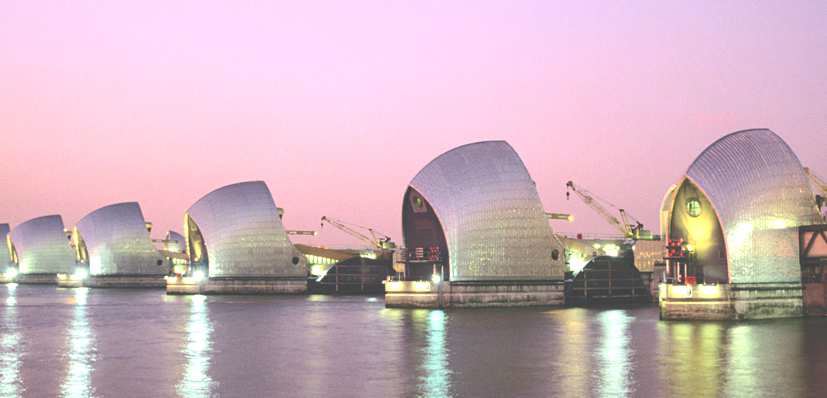
\includegraphics[width=.7\linewidth]{fig_00}
}%figues de la page de garde


\input{\repRel/Style/pagegarde_TD}

\setlength{\columnseprule}{.1pt}

\pagestyle{fancy}
\thispagestyle{plain}

\vspace{5.2cm}


\def\columnseprulecolor{\color{bleuxp}}
\setlength{\columnseprule}{0.4pt} 

%%%%%%%%%%%%%%%%%%%%%%%

\setcounter{numques}{0}

\ifprof
%\begin{multicols}{2}
\else
\begin{multicols}{2}
\fi


\section*{Barrière sur la Tamise}

Le barrage sur la Tamise permet de protéger Londres des grandes marrées évitant ainsi des crues qui pourraient survenir. Ce barrage est constituée de dix portes dont une modélisation est donnée ci-dessous.

\begin{center}
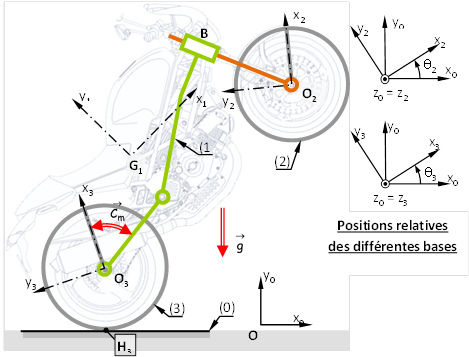
\includegraphics[width=\linewidth]{fig_01}
\end{center}

On donne :
\begin{itemize}
\item $L=\SI{58}{m}$ la longueur de la porte;
\item $R=\SI{12,4}{m}$ le rayon de la porte;
\item $e=\SI{0,05}{m}$ l'épaisseur de la porte, considérée négligeable devant $R$;
\item $\rho=\SI{7800}{kg.m^{-3}}$;
\item $\alpha=\dfrac{\pi}{3}$.
\end{itemize}

%\section*{Présentation du support du cours du cours}

\question{Déterminer les coordonnées du centre d'inertie de la porte : }\textit{
\begin{enumerate}
\item déterminer les coordonnées du centre d'inertie $G_P$ de la plaque;
\item déterminer les coordonnées du centre d'inertie $G_C$ de la portion cylindrique;
\item déterminer les coordonnées du centre d'inertie $G$ de la porte.
\end{enumerate}}

\question{Déterminer la forme de la matrice d'inertie de la porte :}\textit{
\begin{enumerate}
\item donner la forme de la matrice d'inertie de la plaque $P$ en $G_P$;
\item donner la forme de la matrice d'inertie du cylindre $C$ en $G_C$;
\item donner la forme de la matrice d'inertie de la porte $P$ en $G$.
\end{enumerate}}

\question{Déterminer la moment d'inertie de la porte par rapport à $\axe{O}{z}$.}


\ifprof
\else
\end{multicols}
\fi

\newpage

\section*{Matrices d'inertie}
\subparagraph*{}\textit{Donner les formes des matrices d'inertie suivantes.}

\begin{center}
\begin{tabular}{|c|p{2cm}||c|p{2cm}|}
\hline 
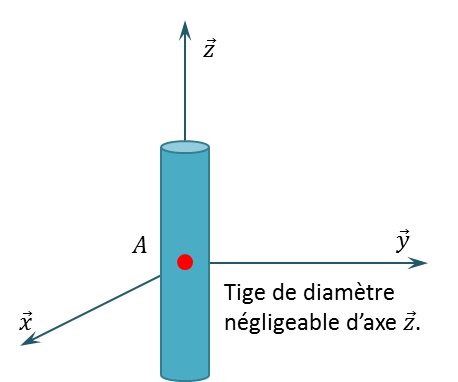
\includegraphics[width=2.8cm]{qcm/Fig_01} & & 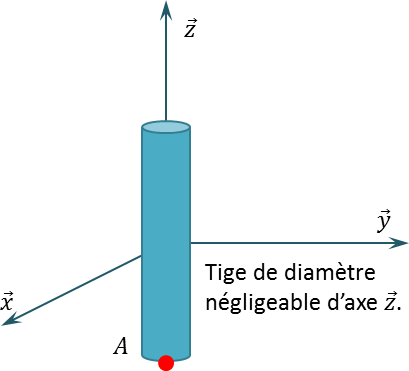
\includegraphics[width=2.8cm]{qcm/Fig_02} & \\ \hline
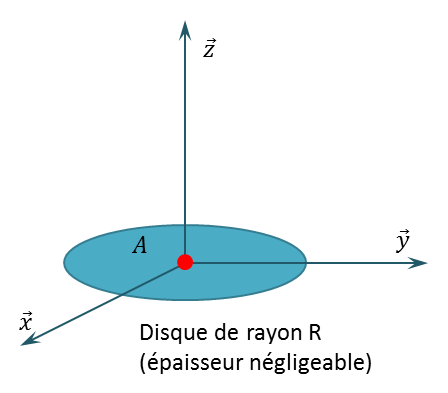
\includegraphics[width=2.8cm]{qcm/Fig_04} & & 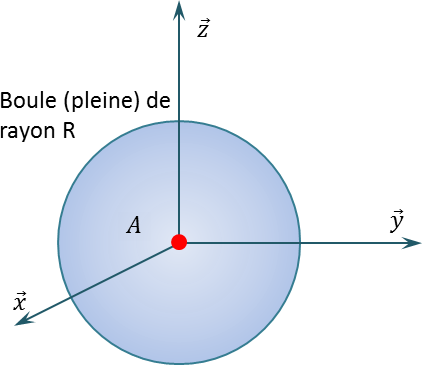
\includegraphics[width=2.8cm]{qcm/Fig_05} & \\ \hline
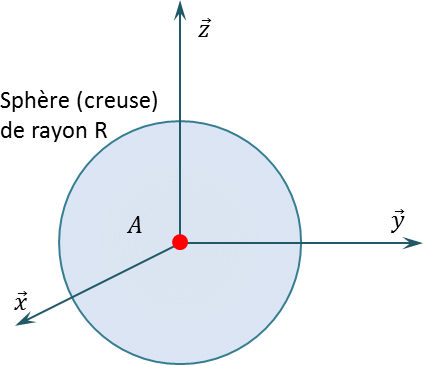
\includegraphics[width=2.8cm]{qcm/Fig_06} & & 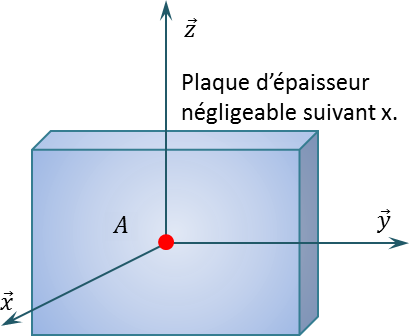
\includegraphics[width=2.8cm]{qcm/Fig_07} & \\ \hline
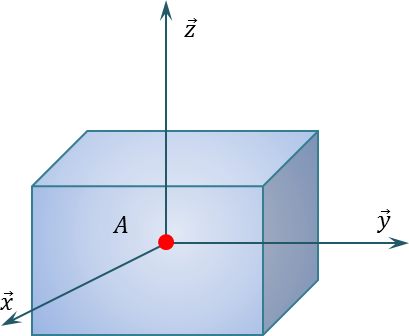
\includegraphics[width=2.8cm]{qcm/Fig_08} & & 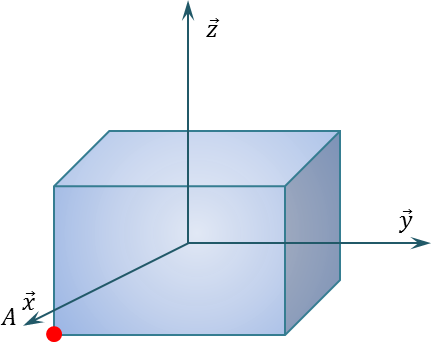
\includegraphics[width=2.8cm]{qcm/Fig_09} & \\ \hline
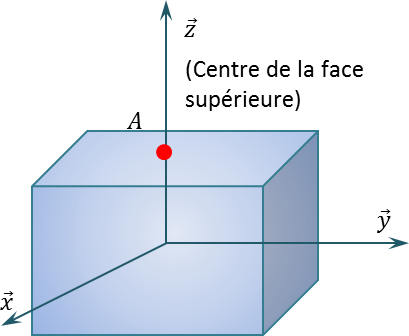
\includegraphics[width=2.8cm]{qcm/Fig_10} & & 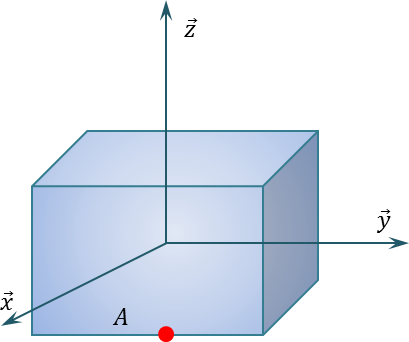
\includegraphics[width=2.8cm]{qcm/Fig_11} & \\ \hline
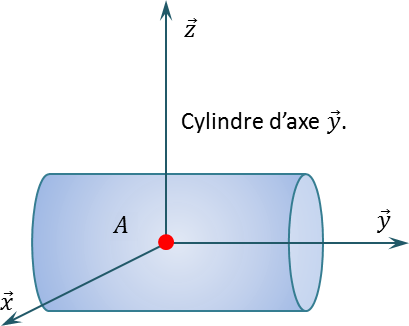
\includegraphics[width=2.8cm]{qcm/Fig_12} & & 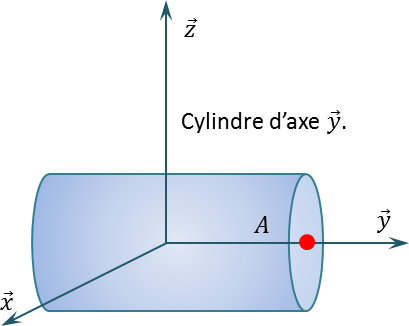
\includegraphics[width=2.8cm]{qcm/Fig_13} & \\ \hline
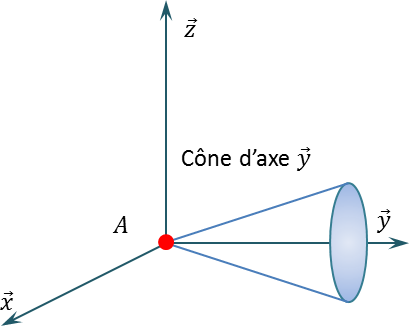
\includegraphics[width=2.8cm]{qcm/Fig_14} & & 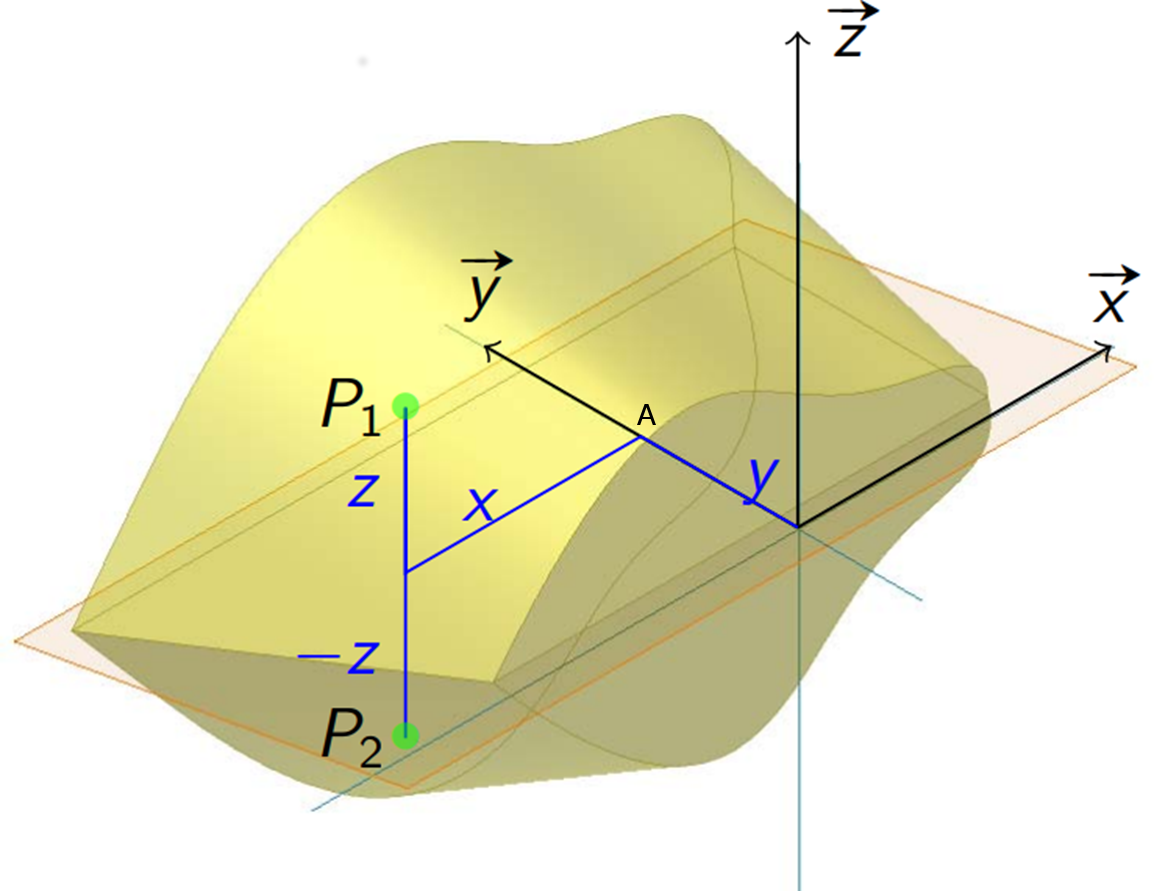
\includegraphics[width=2.8cm]{qcm/Fig_15} & \\ \hline
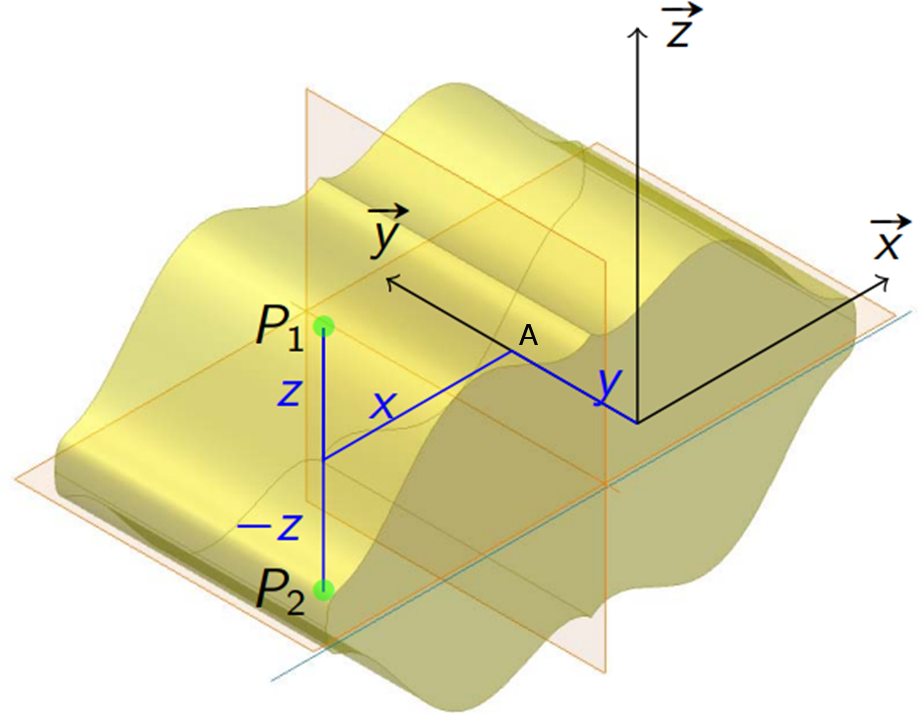
\includegraphics[width=2.8cm]{qcm/Fig_16} & & 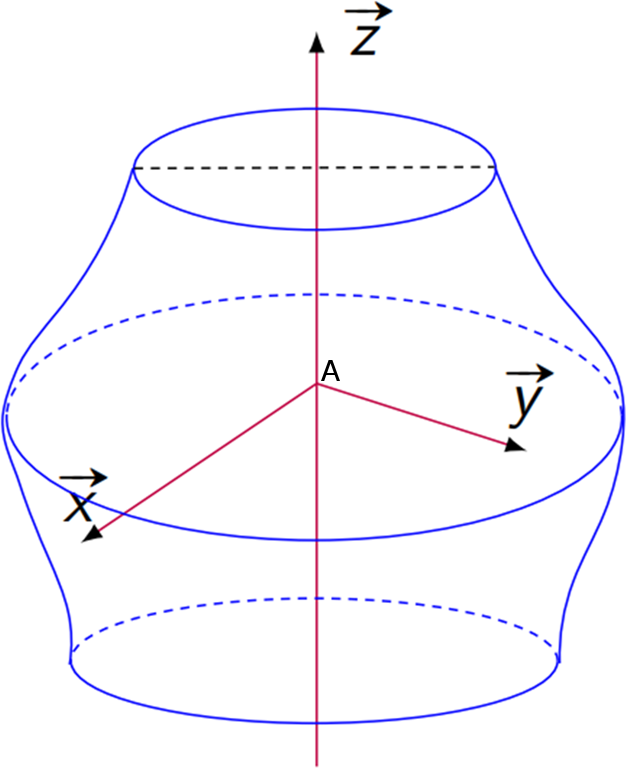
\includegraphics[width=2.8cm]{qcm/Fig_17} & \\ \hline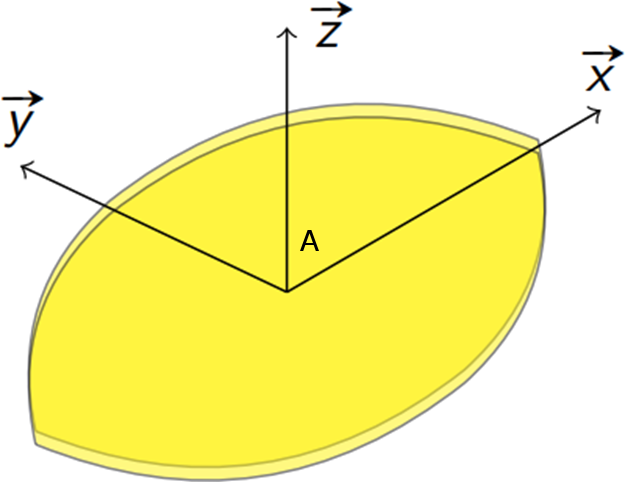
\includegraphics[width=2.8cm]{qcm/Fig_18} & &  & \\ \hline
\end{tabular}
\end{center}

